


\begin{markdown}
#### List of Case Templates
Access to the list by opening the Organisation menu, then the Templates tab, and the Cases tab.
\end{markdown}

\begin{figure}[H]
    \centering
    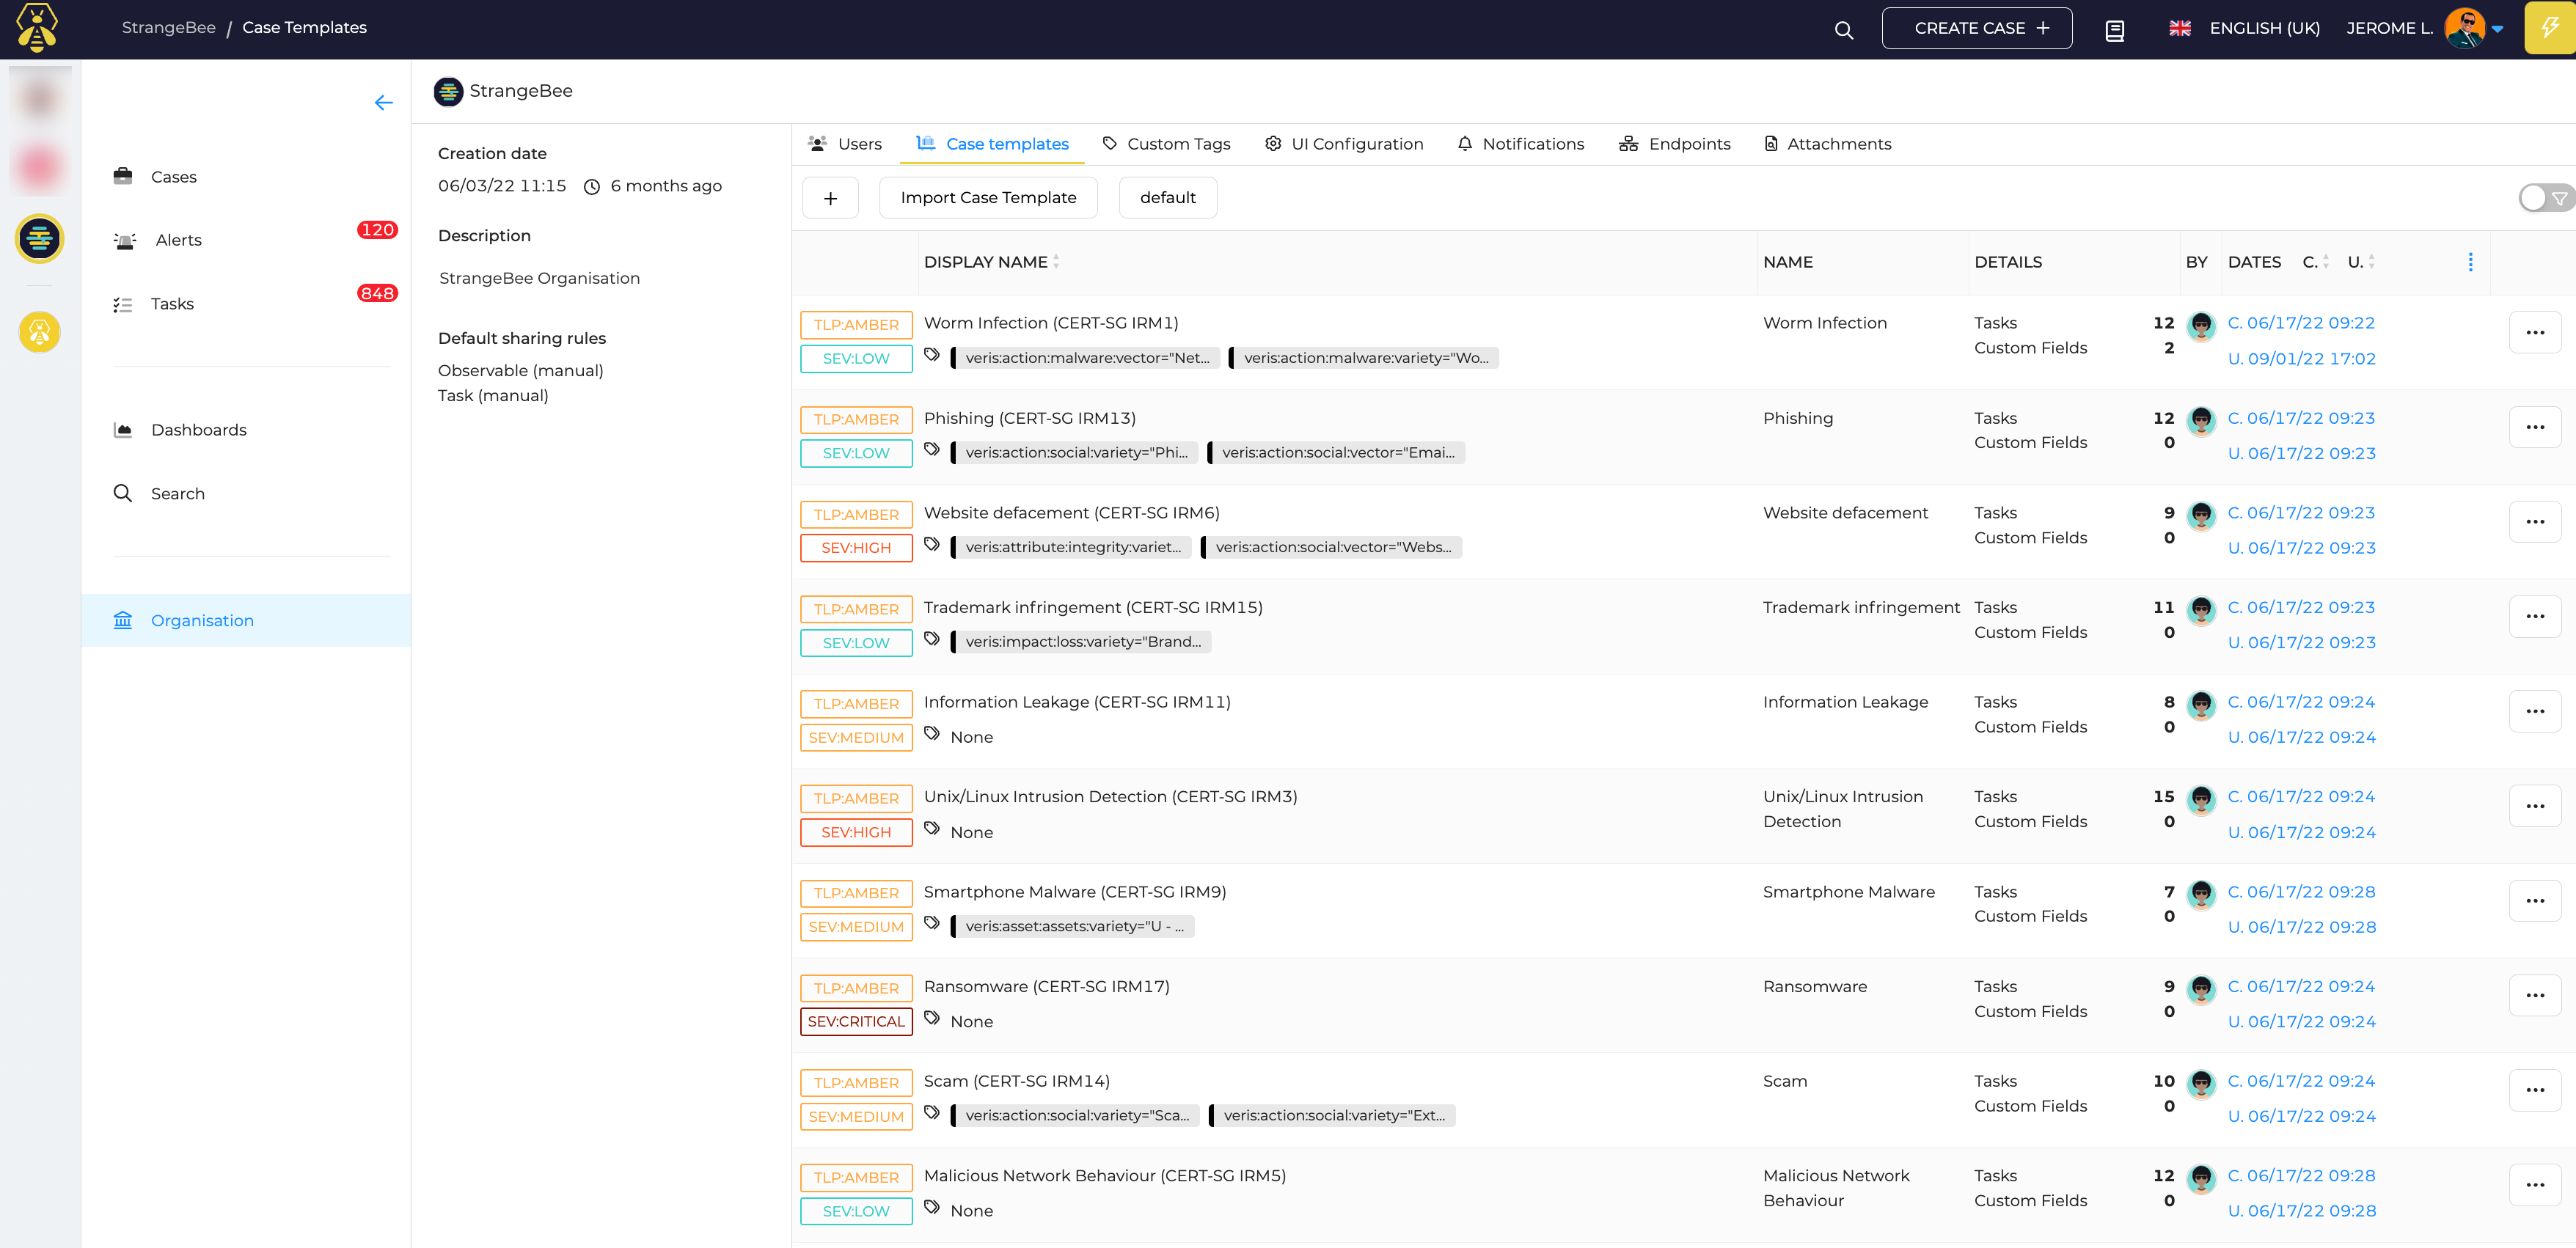
\includegraphics[width=\textwidth]{images/docs/org_admin/templates/case/organisation-case-templates.png}
    \caption{List of case templates}
    \label{fig:modules}
\end{figure}

\begin{markdown}

#### New Case template
Click the + button to create a new Case template.
\end{markdown}



\begin{figure}[H]
    \centering
    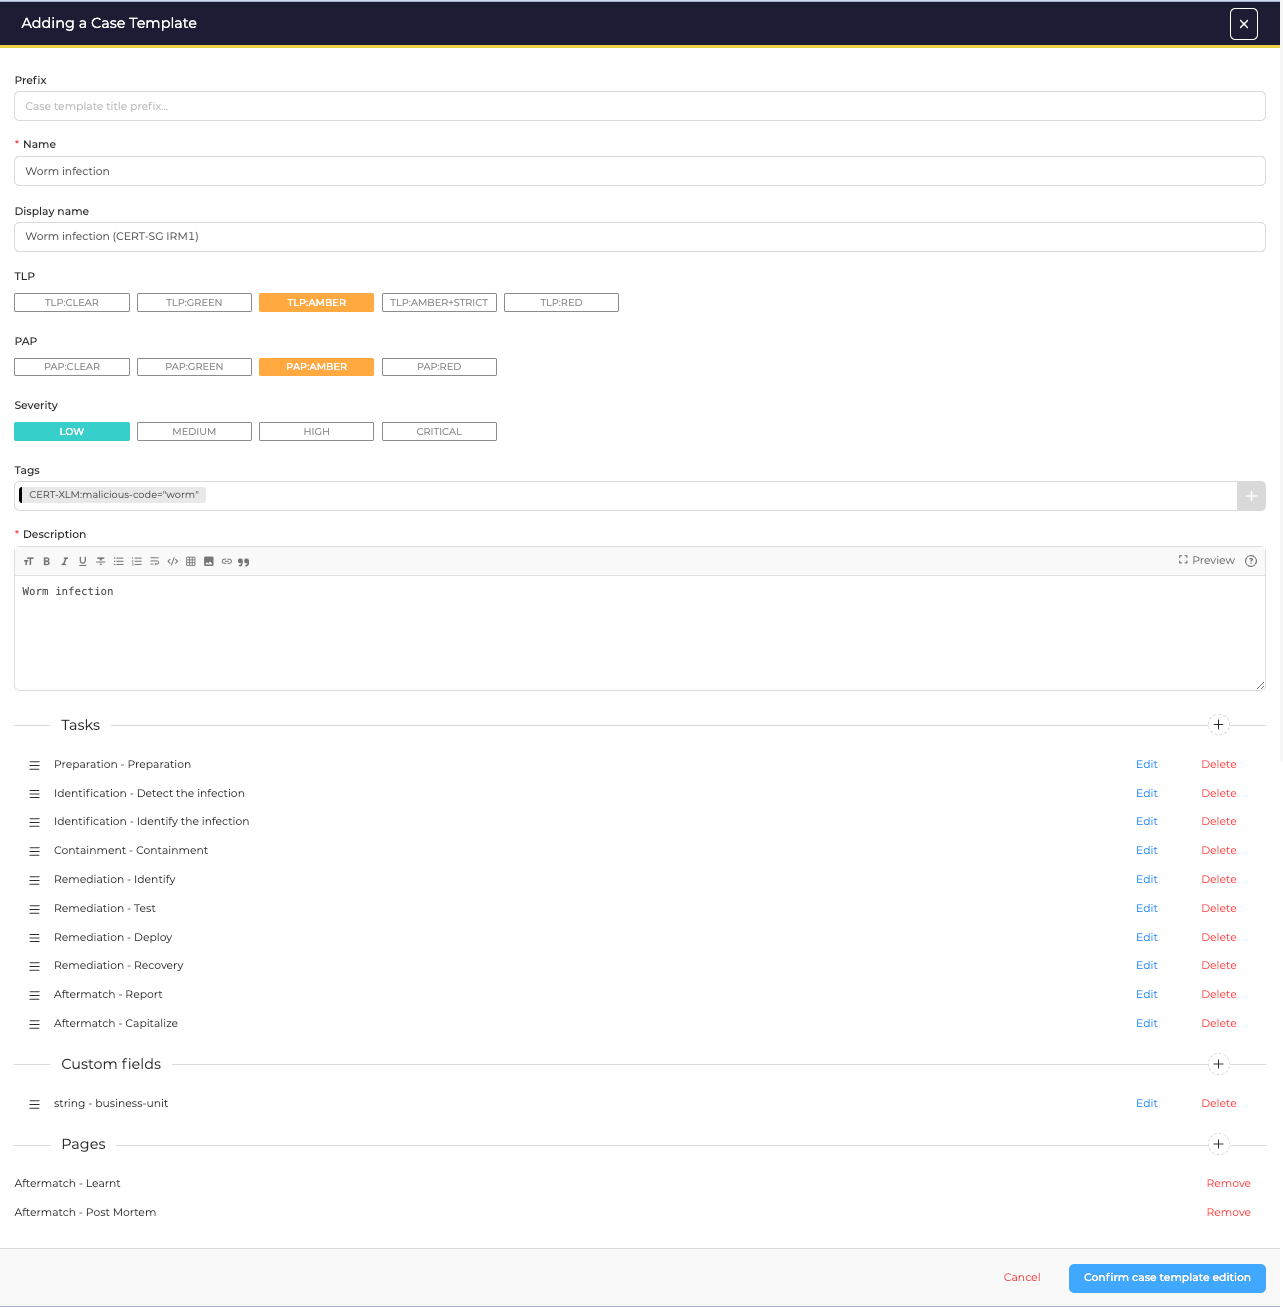
\includegraphics[width=\textwidth]{images/docs/org_admin/templates/case/organisation-case-templates-2.png}
    \caption{New case template}
    \label{fig:modules}
\end{figure}


Configuration parameters#
Prefix
String that will be prepended to the title of a Case when created with this template
Name
Name of the Case template. Used to identify the Case template with the API
Display Name
Name of the Case template displayed in the UI
TLP
Default TLP of the Case when created with this template
PAP
Default PAP of the Case when created with this template
Severity
Default Severity of the Case when created with this template
Tags
List of tags that will be added to the Cases created with this template
Description
Default description of Cases created with this template if not modified.
Tasks
Add tasks to the templates. They will be automatically added to the Case when created with this template
Custom Fields
Add Custom fields to the template. Default value can be set for Custom fields as well.
Pages
Add pages template to the template. They will be automatically added to the Case when created with this template


% #### User management
% Accounts can be deleted or locked, only in the current organisation.
% \end{markdown}